After the C++ adaptation of GASE, the demonstrator for BWA-MEM and GASAL2 integration, we obtained a valid version of BWA-MEM processing sequences in batches, originating from GASE-GASAL2.

BWA-MEM operates with the seed-extension paradigm, and GASAL2 can run the extension part. For a single query sequence, a variable number of seeds can be found. 

For every seed found in the query, the target sequences is the region in the genome around the seed location. Its length is around 1.3 times the length of the query sequence. The extension step is then either:

\begin{itemize}
	\item skipped, meaning that the seed is exactly the size of the sequence,
	\item or done only on one side, if the seed is located at the beginning or the end of the query sequence,
	\item or done on both sides, if the seed is in the middle of the sequence.
\end{itemize}

Most of the time, both sides have to be extended. We create two GPU batches. A simple approach would be to define a batch for the left side, and one for the right side. However, there is an optimised way to split the alignments between two batches.

To avoid divergence, sequences aligned by the GPU threads in the same warp should have similar lengths.  But if one seed is located on the far left and another one on the right, knowing that all queries have the same length, the left parts of the extension will have very different lengths, as shown on Figure~\ref{fig:seds-different-chains}. Moreover, the processing time will be limited by the length of its longest alignment in the GPU batch.
\begin{figure}[h!]
	\centering
	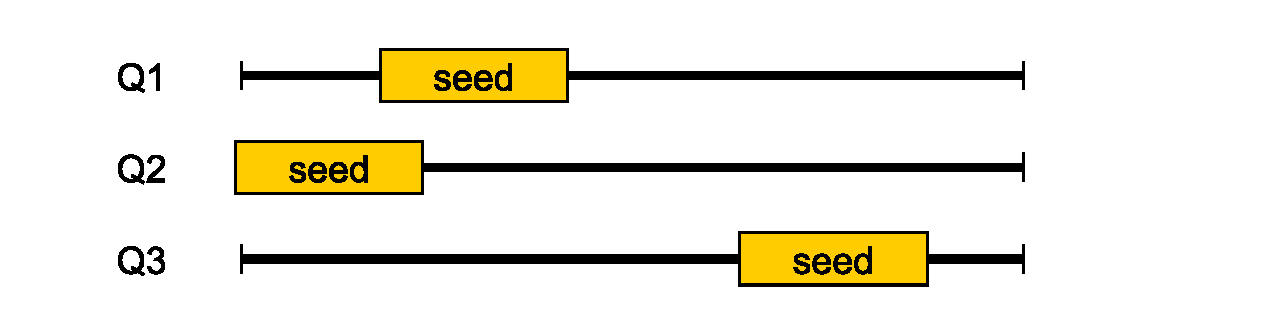
\includegraphics[width=0.7\linewidth]{seds-different-chains}
	\caption{Illustration of chains (in yellow) being located on different places}
	\label{fig:seds-different-chains}
\end{figure}

To summarize, we note that :
\begin{itemize}
	\item all queries have the same length,
	\item the final score is equal to the sum of the chain score, the left part score, and the right part score,
	\item to that extent, we don't need to know whose score is the left one and the right one (only the sum matters),
	\item and we would like to process both sides in parallel.
\end{itemize}

So instead of using two batches for left and right extension, we use two batches for long and short extension. This puts the long sides together to minimise thread divergence. The difference between the longest and the shortest extension in each batch is now at most half the length of the query sequence. For each chain, we log in a dedicated data structure if it has zero, one or two alignments, and on which part (left or right) the long alignment is. When both the "long" and "short" batches of extension are done, the scores are gathered.

Another problem arises: the seeds may have zero, one or two extensions, the short and long batches can have a different number of extension to make. To show this with an example, we can assume that we have three seeds as in Figure~\ref{fig:seds-different-chains}. For the sake of conciseness, only query sequences have been shown, but assume each of these queries have a corresponding target sequence with the same seed located in it, forming pairs of query-target sequences. Chains from Q1, Q2 and Q3 are found in this order, and the \verb|gpu_storage| structure is filled in this order too. Table~\ref{tbl:batches} shows how the batches are filled for this case. Notice that the number of sequences are not the same in two batches, hence two sides of the same alignments are not at the same index on both structures. To circumvent this problem we added information in the data structure of BWA-MEM containing the alignment scores. After both sides of the seed-extension of a batch are finished, this data structure is used to know how many alignments for a seed were computed, ensuring correct gathering. This is not an issue in the original software as the seed is extended first to the right and then to the left. But in our implementation we run both the extensions in parallel, with seed score as the starting score of the alignment, to extract more parallelism  So if we sum both left and right scores, we count the seed score twice. Therefore, we subtract the seed score from the total of extension scores of left and right side . When only one extension is made (or none), we do not have to do this subtraction.

\begin{table}
	\centering
	\begin{tabular}{|c|c|}
		\hline 
		\textbf{``Long" batch} & \textbf{``Short" batch} \\ 
		\hline 
		Pair 1, right part & Pair 1, left part \\ 
		\hline 
		Pair 2, right part & Pair 3, right part \\ 
		\hline 
		Pair 3, left part &  \\ 
		\hline 
	\end{tabular} 
	\caption{Example of how batches are filled.}
	\label{tbl:batches}
\end{table}

